\chapter{Introducción}
\thispagestyle{empty}


\section{Marco temático: esculturas cinéticas}
\subsection{Definición}
Las esculturas cinéticas (kinetic sculpture en inglés) son estructuras tridimensionales en donde el movimiento es una parte fundamental del conjunto. Para lograr el efecto de movimiento en el espacio estos sistemas se construyen con partes móviles que pueden cambiar de posición ya sea naturalmente por acción del viento, como se ve en la figura \ref{fig:1.1}, o de manera forzada. \\
% https://www.youtube.com/watch?v=D2HF-1xjpP8

\begin{figure}[!ht]
	\centering
	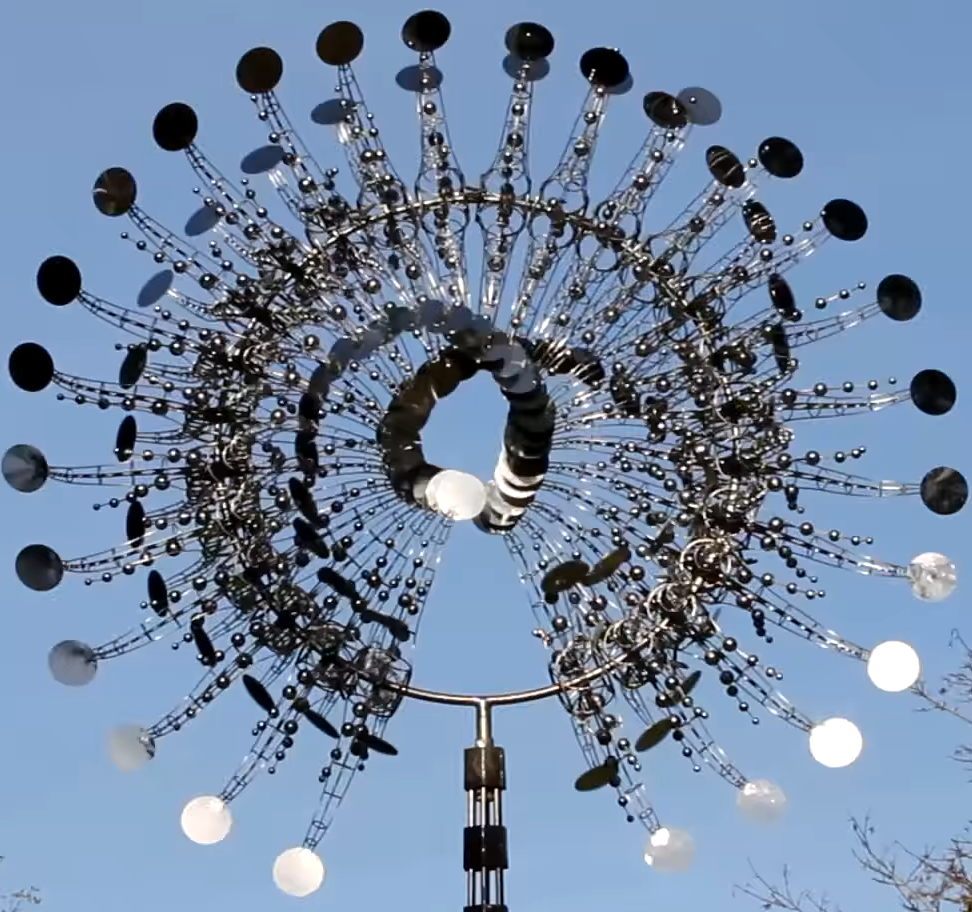
\includegraphics[width=12cm,scale=1]{resources/4-kinSculp1.png}
	\caption{ Ejemplo de escultura cinética movida por aire, por Anthony Howe. \href{https://www.youtube.com/watch?v=N-1LpikCSR4}{LINK al video} }
	\label{fig:\thefigure}
\end{figure}

\subsection{Aplicaciones y estado actual del arte}
Al ser obras que caen dentro del campo artístico suelen presentarse en museos y utilizarse para fines decorativos ya sea en parques o eventos. Sin embargo, el nivel de ingeniería y diseño que algunas de ellas requieren las tornan un interesante desafío intelectual y creativo.\\


Las aplicaciones puntuales de estructuras cinéticas a las que se hará foco en este informe, debido a la naturaleza del proyecto final, son aquellas en donde el efecto espacial se logra a través del movimiento en el eje vertical de objetos esféricos mediante motores. \\


Un ejemplo de aplicación de estas características se puede ver en la figura \ref{fig:1.2}. Allí se muestra una escultura presentada en el Museo de BMW, en Munich, Alemania, en donde 714 esféras metálicas son coordinadas para formas figuras como olas, gotas, y hasta la silueta de un auto \\
\begin{figure}[!ht]
	\centering
	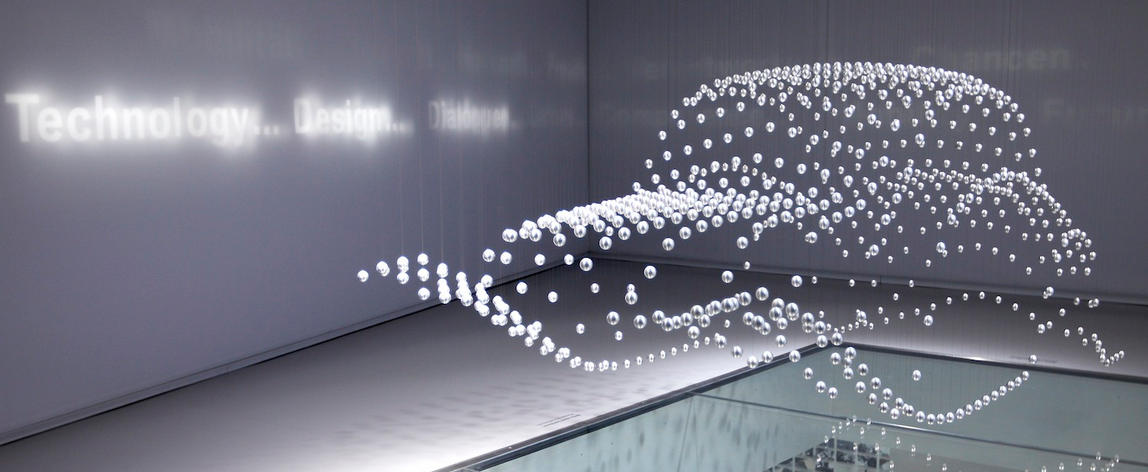
\includegraphics[width=15cm,scale=1]{resources/4-kinSculp2.png}
	\caption{ Escultura cinética en el museo BMW. \href{https://www.youtube.com/watch?v=HVhVClFMg6Y}{LINK al video} }
	\label{fig:\thefigure}
\end{figure}

Otro ejemplo de aplicación se puede ver en la figura \ref{fig:1.3}, en una obra presentada por la empresa Build Up en un centro comercial en Fukuoka, Japón. Allí se instalaron 1000 luminarias esféricas RGB dispuestas en una matriz de 25x40 para generar figuras tridimensionales como planos y gausseanas, entre otras. \\
\begin{figure}[!ht]
	\centering
	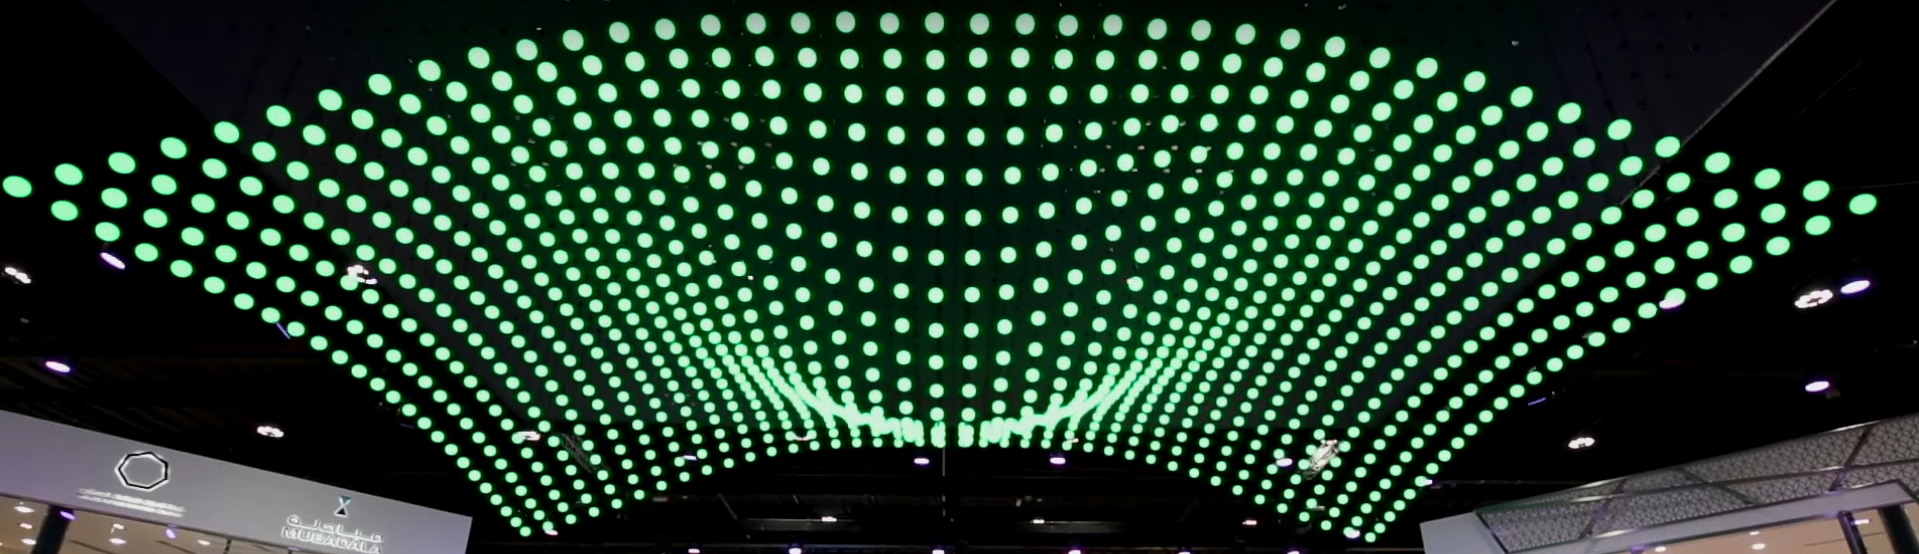
\includegraphics[width=15cm,scale=1]{resources/4-kinSculp3.png}
	\caption{ Escultura cinética por parte de Build Up. \href{https://www.youtube.com/watch?v=ICixCazf6-k}{LINK al video} }
	\label{fig:\thefigure}
\end{figure}

\newpage
En el caso del último ejemplo presentado los efectos espaciales se logran coordinando el movimiento de cada esfera independientemente, cada una manejada por un equipo motorizado. Para esto un profesional capacitado indica, cual director de orquesta, la posición, velocidad y colores de cada esfera en un programa que es ejecutado por una consola de control de iluminación, como pueden ser las consolas hog 4 de \href{https://www.highend.com/}{High End Systems}. La comunicación entre dicha consola y los equipos se realiza a través del protocolo \textbf{DMX}.

\section{DMX}
\subsection{definición}
DMX es un protocolo comúnmente utilizado para el manejo de luminarias que emplea el estándar EIA-485 como capa física y paquetes de largo variable para la comunicación entre maestro y esclavo (que suele ser unidireccional).
\subsection{Capa física}
tipo de señal, canal físico

\subsection{Capa de enlace de datos}
canales, addressamiento
\subsection{Equipos que implementan DMX}


\section{Updown}
\subsection{Definición}


\subsection{Blackout}
Black-out es una empresa productora y proveedora de tecnología, cuyo objetivo es generar contenido audiovisual para grandes eventos. Para cumplir con este objetivo la empresa dedica recursos al desarrollo de productos tecnológicos innovadores, como es el caso de los equipos destinados a generar las llamadas Esculturas cinéticas (Kinetic sculpture en inglés).\\

\subsection{Productos que compiten en el mercado}
El equipos más conocido para estas aplicaciones es el \href{http://www.eastsunlite.com/p31.html}{OrbisFly}, de \href{https://www.kinetic-lights.com/}{Kinetic Lights}. Estos dispositivos de origen Chino trabajan con una esfera RGB de peso estándar de 1Kg, aunque soporta un peso máximo de 2Kg, que puede descender hasta 9 metros. Dispone de un display LCD y botoneras para el testeo y configuración el equipo\\




\newpage
\section{Justificación del proyecto}
La empresa Black-out se encargó de comenzar el desarrollo de los Up-down; los equipos necesarios para crear los efectos de esculturas cinéticas. El inconveniente es que solo fue armada la parte mecánica del mismo, ya que a efectos prácticos el firmware que se utilizaba para manejar el conjunto era pobre.\\
Ante la necesidad que se tiene que el equipo controle la posición y velocidad de la carga, y que además verifique errores de hardware durante su uso para evitar accidentes, surgió la necesidad de buscar a alguien capacitado para mejorar la programación y terminar el proyecto.
Es entonces que se presentó la oportunidad de realizar un trabajo en la empresa con el objetivo de completar lo que falta del proyecto, hacer que este cumpla ciertas especificaciones técnicas, y crear documentación sobre el firmware y software de prueba de hardware para que más equipos de las mismas características puedan ser producidos. De esta manera, para completar el objetivo se debe:
\begin{itemize}
	\item Implementar un control automático de posición y velocidad de la carga movida por el equipo para lograr los efectos deseados.
	\item Permitir el cambio de los setpoints de posición y velocidad mediante comandos DMX enviados al equipo por una consola de luces, como puede ser una \href{https://www2.highend.com/products/controllers/Hog4Console.asp}{consola HOG4}
	\item Manejar errores y excepciones de hardware para lograr que el producto sea seguro, siendo que será instalado en eventos con un alto nivel de concurrencia.
\end{itemize}




